\documentclass[jou, noextraspace]{apa6}

\usepackage{tcolorbox}
\usepackage{ulem} %math
\usepackage{amsmath}
\usepackage{amsfonts}
\usepackage{amssymb}
\usepackage{graphicx}
\usepackage{enumerate}


%Create a box for theorems
%\begin{theo}[titel] %optional
%tekst
%\end{theo}
\newenvironment{theo}[1][Vigtigt]{%
\begin{tcolorbox}[colback=green!5,colframe=green!40!black,title=\textbf{#1}]
}{%
\end{tcolorbox}
}




%Create a square matrix
%\begin{ArgMat}{2}
%21 & 22 & 23 \\  
%a & b & c
%\end{ArgMat}
%
% Info: http://tex.stackexchange.com/questions/2233/whats-the-best-way-make-an-augmented-coefficient-matrix
%
\newenvironment{ArgMat}{%
$
  \left[\begin{array}{@{}*{100}{r}r@{}}
}{%
  \end{array}\right]
  $
}

\newenvironment{deter}{%
$
  \left|\begin{array}{@{}*{100}{r}r@{}}
}{%
  \end{array}\right|
  $
}


%Create multiple lines with holes
%\begin{SysEqu}
%x_1 && &- &5x_3 &+ &2x_4=& 1 \\
%x_1 &+ &x_2 &+ &x_3 && =& 4 \\
%&&&&&&0 =& 0
%\end{SysEqu}
\newenvironment{SysEqu}{%
$  \setlength\arraycolsep{0.1em}
  \begin{array}{@{}*{100}{r}r@{}}
}{%
  \end{array}$
}

%Create solution for x_1, x_n...
%\begin{solu}
%x_1 &= d \\
%x_2 &= e \\
%x_3 &= s
%\end{solu}
\newenvironment{solu}{%
$
  \setlength\arraycolsep{0.1em}
  \left\{\begin{array}{@{}*{100}{r}r@{}}
}{%
  \end{array}\right.
$
}

\usepackage{lastpage}


\newcommand{\HRule}{\rule{\linewidth}{0.8mm}}

%Tekst i fotter
\newcommand{\footerText}{\thepage\xspace /\pageref{LastPage}}
\newcommand{\ProjectName}{433 MHz styring af AeroQuad}


\chapterstyle{hangnum}




\nouppercaseheads
\makepagestyle{mystyle} 

\makeevenhead{mystyle}{}{\\ \leftmark}{} 
\makeoddhead{mystyle}{}{\\ \leftmark}{} 
\makeevenfoot{mystyle}{}{\footerText}{} 
\makeoddfoot{mystyle}{}{\footerText}{} 
\makeatletter
\makepsmarks{mystyle}{% Overskriften på sidehovedet
  \createmark{chapter}{left}{shownumber}{\@chapapp\ }{.\ }} 
\makeatother
\makefootrule{mystyle}{\textwidth}{\normalrulethickness}{0.4pt}
\makeheadrule{mystyle}{\textwidth}{\normalrulethickness}

\makepagestyle{plain}
\makeevenhead{plain}{}{}{}
\makeoddhead{plain}{}{}{}
\makeevenfoot{plain}{}{\footerText}{}
\makeoddfoot{plain}{}{\footerText}{}
\makefootrule{plain}{\textwidth}{\normalrulethickness}{0.4pt}

\pagestyle{mystyle}

%%----------------------------------------------------------------------
%
%%Redefining chapter style
%%\renewcommand\chapterheadstart{\vspace*{\beforechapskip}}
%\renewcommand\chapterheadstart{\vspace*{10pt}}
%\renewcommand\printchaptername{\chapnamefont }%\@chapapp}
%\renewcommand\chapternamenum{\space}
%\renewcommand\printchapternum{\chapnumfont \thechapter}
%\renewcommand\afterchapternum{\space: }%\par\nobreak\vskip \midchapskip}
%\renewcommand\printchapternonum{}
%\renewcommand\printchaptertitle[1]{\chaptitlefont #1}
\setlength{\beforechapskip}{0pt} 
\setlength{\afterchapskip}{0pt} 
%\setlength{\voffset}{0pt} 
\setlength{\headsep}{25pt}
%\setlength{\topmargin}{35pt}
%%\setlength{\headheight}{102pt}
%\setlength{\textheight}{302pt}
\renewcommand\afterchaptertitle{\par\nobreak\vskip \afterchapskip}
%%----------------------------------------------------------------------




%Sidehoved og -fod pakke
%Margin
\usepackage[left=2cm,right=2cm,top=2.5cm,bottom=2cm]{geometry}
\usepackage{lastpage}



%%URL kommandoer og sidetal farve
%%Kaldes med \url{www...}
%\usepackage{color} %Skal også bruges
\usepackage{hyperref}
\hypersetup{ 
	colorlinks	= true, 	% false: boxed links; true: colored links
    urlcolor	= blue,		% color of external links
    linkcolor	= black, 	% color of page numbers
    citecolor	= blue,
}



%Mellemrum mellem linjerne    
\linespread{1.5}


%Seperated files
%--------------------------------------------------
%Opret filer således:
%\documentclass[Navn-på-hovedfil]{subfiles}
%\begin{document}
% Indmad
%\end{document}
%
% I hovedfil inkluderes således:
% \subfile{navn-på-subfil}
%--------------------------------------------------
\usepackage{subfiles}

%Prevent wierd placement of figures
%\usepackage[section]{placeins}

%Standard sti at søge efter billeder
%--------------------------------------------------
%\begin{figure}[hbtp]
%\centering
%\includegraphics[scale=1]{filnavn-for-png}
%\caption{Titel}
%\label{fig:referenceNavn}
%\end{figure}
%--------------------------------------------------
\usepackage{graphicx}
\usepackage{subcaption}
\usepackage{float}
\graphicspath{{../Figures/}}

%Speciel skrift for enkelt linje kode
%--------------------------------------------------
%Udskriver med fonten 'Courier'
%Mere info her: http://tex.stackexchange.com/questions/25249/how-do-i-use-a-particular-font-for-a-small-section-of-text-in-my-document
%Eksempel: Funktionen \code{void Hello()} giver et output
%--------------------------------------------------
\newcommand{\code}[1]{{\fontfamily{pcr}\selectfont #1}}


% Følgende er til koder.
%----------------------------------------------------------
%\begin{lstlisting}[caption=Overskrift på boks, style=Code-C++, label=lst:referenceLabel]
%public void hello(){}
%\end{lstlisting}
%----------------------------------------------------------

%Exstra space
\usepackage{xspace}
%Navn på bokse efterfulgt af \xspace (hvis det skal være mellemrum
%gives det med denne udvidelse. Ellers ingen mellemrum.
\newcommand{\codeTitle}{Kodeudsnit\xspace}

%Pakker der skal bruges til lstlisting
\usepackage{listings}
\usepackage{color}
\usepackage{textcomp}
\definecolor{listinggray}{gray}{0.9}
\definecolor{lbcolor}{rgb}{0.9,0.9,0.9}
\renewcommand{\lstlistingname}{\codeTitle}
\lstdefinestyle{Code}
{
	keywordstyle	= \bfseries\ttfamily\color[rgb]{0,0,1},
	identifierstyle	= \ttfamily,
	commentstyle	= \color[rgb]{0.133,0.545,0.133},
	stringstyle		= \ttfamily\color[rgb]{0.627,0.126,0.941},
	showstringspaces= false,
	basicstyle		= \small,
	numberstyle		= \footnotesize,
%	numbers			= left, % Tal? Udkommenter hvis ikke
	stepnumber		= 2,
	numbersep		= 6pt,
	tabsize			= 2,
	breaklines		= true,
	prebreak 		= \raisebox{0ex}[0ex][0ex]{\ensuremath{\hookleftarrow}},
	breakatwhitespace= false,
%	aboveskip		= {1.5\baselineskip},
  	columns			= fixed,
  	upquote			= true,
  	extendedchars	= true,
 	backgroundcolor = \color{lbcolor},
	lineskip		= 1pt,
%	xleftmargin		= 17pt,
%	framexleftmargin= 17pt,
	framexrightmargin	= 0pt, %6pt
%	framexbottommargin	= 4pt,
}

%Bredde der bruges til indryk
%Den skal være 6 pt mindre
\usepackage{calc}
\newlength{\mywidth}
\setlength{\mywidth}{\textwidth-6pt}


% Forskellige styles for forskellige kodetyper
\usepackage{caption}
\DeclareCaptionFont{white}{\color{white}}
\DeclareCaptionFormat{listing}%
{\colorbox[cmyk]{0.43, 0.35, 0.35,0.35}{\parbox{\mywidth}{\hspace{5pt}#1#2#3}}}
\captionsetup[lstlisting]
{
	format			= listing,
	labelfont		= white,
	textfont		= white, 
	singlelinecheck	= false, 
	width			= \mywidth,
	margin			= 0pt, 
	font			= {bf,footnotesize}
}

\lstdefinestyle{Code-C} {language=C, style=Code}
\lstdefinestyle{Code-Java} {language=Java, style=Code}
\lstdefinestyle{Code-C++} {language=[Visual]C++, style=Code}
\lstdefinestyle{Code-VHDL} {language=VHDL, style=Code}
\lstdefinestyle{Code-Bash} {language=Bash, style=Code}

%Text typesetting
%--------------------------------------------------------
%\usepackage{baskervald}
\usepackage{lmodern}
\usepackage[T1]{fontenc}              
\usepackage[utf8]{inputenc}         
\usepackage[english]{babel}       

\setlength{\parindent}{0pt}
\nonzeroparskip

%\setaftersubsecskip{1sp}
%\setaftersubsubsecskip{1sp}
 


%Dybde på indholdsfortegnelse
%----------------------------------------------------------
%Chapter, section, subsection, subsubsection
%----------------------------------------------------------
\setcounter{secnumdepth}{3}
\setcounter{tocdepth}{3}


%Tables
%----------------------------------------------------------
\usepackage{tabularx}
\usepackage{array}
\usepackage{multirow} 
\usepackage{multicol} 
\usepackage{booktabs}
\usepackage{wrapfig}
\renewcommand{\arraystretch}{1.5}



%Misc
%----------------------------------------------------------
\usepackage{cite}
\usepackage{appendix}
\usepackage{amssymb}
\usepackage{url,ragged2e}
\usepackage{enumerate}
\usepackage{amsmath} %Math bibliotek


\usepackage{longtable}



%BibLatex
\usepackage[style=ieee, sortcites=false, backend=biber, block=ragged]{biblatex} 
\DeclareLanguageMapping{american}{american-ieee} %BibLatex mapping
\addbibresource{References.bib}

\bibsetup{
	\setcounter{abbrvpenalty}{0}
	\setcounter{highnamepenalty}{0}
	\setcounter{lownamepenalty}{0}
}

% \usepackage{breakcites}

\title{False-Positive Filter in Context-Aware Applications}
\shorttitle{False-Positive Filter in Context-Aware Applications}

\author{Rasmus Bækgaard}
\journal{Aarhus University}
\volume{\today}

\affiliation{Aarhus University}

\leftheader{Bækgaard}
\date{\today}

%!TEX root = Main.tex
% Background
% Objectives
% Methods
% Results
% Discussion/Conclussion
\begin{abstract}
Ambient assisted living systems exists to give mostly elder people certainty, that alerts will be triggered e.g. should they fall in their homes, when wearing a fall detector.
To ensure the data from the fall detector is not a false-positive, a service can be created to plug into an existing system, analyzing other sensors' data to confirm/invalidate the detector's claim.
This article describes how such a service can be designed, plugged into an existing system, and provide a reliable analysis of incoming data.
A proof-of-concept application will be created to show the design is valid and fulfill the requirements of the objective.
Finally the article will elaborate on how proof-of-concept can be even better.

\end{abstract}


\keywords{Fall detection, Context Aware, sensors, Ambient Assisted Living, Pervasive computing, False-positive filter} %shown after abstract

\date{\today}

\begin{document}

\maketitle

%!TEX root = Main.tex
\section{Introduction}

For elder people, one fear of being alone is what will happen if they fall and cannot get up by them self\cite{bell2000characteristics}.
Some nursing homes and sheltered housings have installed sensors of various forms\cite{Tun-Loft}, to detect e.g. a fall in the building and alert personal should a fall occur. 
But sensors that detects falls can be error-prone\cite{bardram2008context} and provide false-positives, which will trigger events that calls for personal to help.
This is most unwanted and should be possible to avoid using data from other sensors, to help determine whether the signal is a false-positive or not.
\\
This paper presents the work from a study for a service that will assist in doing just that.
The aim is to evaluate a feasibility prototype of such a false-positive filter, that will analyze incoming data from various sensors, and thereby determine a probability of false-positive events, based on custom user credentials of what should influent the decision.

% This paper is written based on a Research and Development project for Aarhus University's Engineering Department.
% The project is handling the problem of detecting a false-positive from sensors, when they obviously does not happen, and the given sensor will trigger a critical alarm.
% The case taken in the project is based on a patient wearing a fall detector, and a bed with a 'in-bed' detector.
% Should said patient lie down on the bed and somehow trigger the fall detector, both the fall detector and the 'in-bed' detector will send events of occurrence. 
% But lying down in bed is not a fall, so the system should be able to recognize this as a false-positive from the fall detector.


%!TEX root = Main.tex
\section{Purpose}

To ensure that the scenario can be implemented to an existing system, it is important not to rewrite code of the existing system, but add to it, thus not breaking it for other developers.
The Common Ambient Assisted Living Homecare Platform, CAALHP, is a framework which behaves as a Context-Awareness system, just like the Java Context-Awareness Framework\cite{JCAF}, JCAF.
JCAF is built upon layers to ensure functionality and responsibility is divided to those who should handle it, allowing devices monitoring service by subscribing to them, letting services subscribe to devices and publish data to the monitors.
Another context framework implementing this technique is the Context Toolkit\cite{ContextToolkit}, which consist of several types of class, including \texttt{interpreters} to convert context to higher level information, and \texttt{discoverers} to register capabilities in the framework.

By using an object oriented model, a service for CAALHP (written in C\#) will be able to use inheritance, objects, an encapsulations to represent the data retrieved from the sensor and present them to monitors or other services, much as show on Figure \ref{fig:JCAF}.
The service will be automatically added to the CAALHP with context discoverers.

\begin{figure}[hbtp]
	\centering
	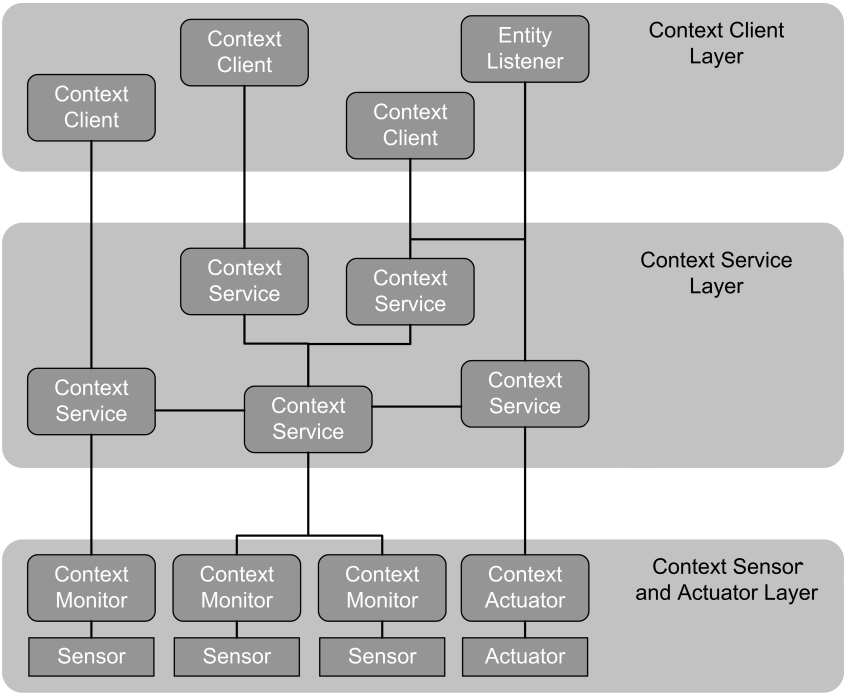
\includegraphics[width = 0.48 \textwidth]{JCAF}
	\caption{JCAF hierarchi\cite[5]{JCAF}. 
	Sensors are monitored by context monitors, which will provide the Context Service Layer with data from the sensors.
	The Context Services can subscribe to any number of Context Monitors and other Context Services, to calculate and present data for Context Clients, which can trigger alarms, display data for a user etc.}
	\label{fig:JCAF}
\end{figure}

The CAALHP is an Open Source project\cite{BB-CAALHP} which already operates with several different sensors and services.
Adding functionality must not affect other parts of the system -- it must run by it self, subscribing to the types of events coming into the system, and providing and API for the data the service handles.



%!TEX root = Main.tex
\section{Method}

% Analysis (hvor du skriver om hvordan du vil undersøge behov og udfordringer)
% Design (hvor du skriver hvilke metoder du vil bruge til at designe)
% Evaluation (hvor du skriver hvordan du vil teste den resulterende funktionsprototype)

\subsection{Analysis}

The false-positive filter can only be build successfully, if it can be validated as actual functional in a scenario.
For this study a Shimmer unit\cite{Shimmer} will be used, since this can be programmed to be a fall detector, and a Carebed\fxnote{Reference to CareBed} will be able to detect when a person is in bed.
But gaining data from hardware is hard to test. 
Letting software fake the input can therefore be designed to provide this data, allowing seamless integration for the hardware tests when a prototype is ready to be tested.

When the Shimmer is activated and sends an event of a fall, the system shall look for whether the CareBed has send any events of a person being in bed within the last ten seconds.
Should this scenario be, the probability of the person actually falling be reduced tremendiously, since the person is in their bed, and not fallen on the floor.
If the Shimmer is actiavted and the CareBed has no records of a person being in the bed, the system shall give a high probability of a fall occurring.

\subsection{Design}

The CAALHP already contains events which are send around in the system; read, modified, and resend.
But the architecture of them does not suite the needs for this service.
Therefore a new type of events must be created to let the service know what is actually send.
The two sensors this project use, the Shimmer and the CareBed, can tell if you are in bed or not, or if you have fallen.
But the sensor will not be sending the same type of data, and other sensors, which will be added in future projects, will very likely send its own different data as well.
Therefore a base type is created with two different inherited classes, a basic and an advanced -- both able to send a list with their own data, but also send either a probability of actual occurrence, since the data could indicate whether it is a 'maybe', or send a simple 'did'/'did not' happen.
The data structure for this can be seen in \codeTitle \ref{lst:BaseEvent}.

\begin{lstlisting}[caption=The BaseEvent class with inherited Basic and Advanced class, style=Code-C++, label=lst:BaseEvent]
public abstract class BaseEvent : Event
{
	public List<int> Data;
	public dynamic Condition;
	public string TimeStamp;

	[BsonId] 
	public Guid Id;

	[BsonConstructor]
	protected BaseEvent()
	{
		CallerProcessId = 0;
		Data = new List<int>();
		Condition = 0;
		TimeStamp = DateTime.Now.ToString();
		Id = Guid.NewGuid();
	}
}

public abstract class Basic : BaseEvent
{
	[BsonConstructor]
	protected Basic() {}
}

public abstract class Advanced : BaseEvent
{
	[BsonConstructor]
	protected Advanced() {}
}
\end{lstlisting}


When data is received, stored and ready to be handled, a fall events must be a fall event, and not just an advanced event, since this actually said nothing of what happened.
Therefore an additional inherited class is created from both the basic and the advance class, to categorize the event as a fall event or as a bed event.
Now the faker services and the real services will be presented as a specific type, and additional services could easily add their own types of events, as seen in \codeTitle \ref{lst:Events}.

\begin{lstlisting}[caption=Inherited classes of the Basic and Advance class., style=Code-C++, label=lst:Events]
public abstract class FallEvent : Advanced
{
	[BsonConstructor]
	protected FallEvent() {}
}

public abstract class BedEvent : Basic
{
	[BsonConstructor]
	protected BedEvent() {}
}

public class CareBed : BedEvent
{
	[BsonConstructor]
	public CareBed() {}
}

public class Shimmer : FallEvent
{
	[BsonConstructor]
	public Shimmer() {}
}
\end{lstlisting}

All data must to be stored for the system to read.
If the system will only be able to detect what happens when a Context Client\cite{JCAF} is online, potential safety warning will never be send (or send falsely).
Storing events in a database as they occur, which can handle all types of events, is crucial for the functionality of the service.
Because the data type the database must register can vary from event to event, it is important the database can handle different data types in the same collection.
Since picking the most optimal database was not part of the project, the popular MongoDB\cite{MongoDB-ref} was chosen.
It did, however, bring its own problems along the way, since it was upgraded from version 1.10 to 2.0 in the beginning of April\cite{MongoDB-update} and the documentation and help on sites as Stackoverflow.com was quite limited.
However that database was, when finally understood, rather easy to navigate through and test on.

MongoDB requires only that it knows what the type is before it is inserted.
This can be handled when the service is started, as seen in the method \code{ListenToEvents(\dots)} in \codeTitle \ref{lst:ListenToEvents}.
When the service is initialized, the developer will specify which events to subscribe to.
By creating a new instance of all the types wanted in \code{SubscribeToAllEvents} the service will be notified each time an event of the specified type is send through, and will register the type inside MongoDB.

\begin{lstlisting}[caption=Registering classes from the EventAnalyzer, style=Code-C++, label=lst:ListenToEvents]
public class EventAnalyser : IServiceCAALHPContract, IEventAnalyser
{
	public void Initialize(IServiceHostCAALHPContract hostObj, int processId)
	{
		Host = hostObj;
		_processId = processId;

		SubscribeToAllEvents();
	}

	private void SubscribeToAllEvents()
	{
		ListenToEvents(new DummyFall());
		ListenToEvents(new DummyBed());
		ListenToEvents(new Shimmer());
		ListenToEvents(new CareBed());

		RegisterHelper.Instance.AddAffection(typeof(FallEvent), typeof(BedEvent), 10);
	}

	private void ListenToEvents(BaseEvent type, string assemblyName = "EventTypes")
	{
		var genericInfo = EventHelper.GetFullyQualifiedNameSpace(SerializationType.Json,
			type.GetType(), assemblyName);
		Host.Host.SubscribeToEvents(genericInfo, _processId);

		RegisterHelper.RegisterNewClass(type);
	}
}
\end{lstlisting}

When registering new events, the developer can specify for the \code{EventAnalyzer}, how much and event will be affected by another event.
Multiple event can be affected by multiple events.
Creating a dictionary of all the event that can be affect (\code{key}), where each entry can be another type with affection value (\code{value}) can be expressed as here:

\begin{lstlisting}[style=Code-C++]
public Dictionary<Type, Dictionary<Type, int>> AffectionTable;
\end{lstlisting}

This can give a huge tree with affection values as the following example:
\vspace{-15pt}
\begin{verbatim}
+ Shimmer
  - DummyBed = 10
  - CareBed = 12
+ DummyFall
  - DummyBed = 23
  - CareBed = 24
...
\end{verbatim}
\vspace{-10pt}
Much like a database lookup, but without the need of specifying index, the algorithm that determines false-positives can look for events affecting an incoming event.
To look for these event the method in \codeTitle \ref{lst:EventsAffectingIt} can be invoked.
This will look for both concrete types and the super class of these.
This also mean, that the developers can insure the code will work in the future, when new concrete implementations of events are added to the system.
Should someone create another type of bed sensor, the system can subscribe to it, as in \codeTitle \ref{lst:ListenToEvents}.

\begin{lstlisting}[caption=Find affection based on input event, style=Code-C++, label=lst:EventsAffectingIt]
public Dictionary<Type, int> EventsAffectingIt(BaseEvent newEvent)
{
	var affects = new Dictionary<Type, int>();

	if (RegisterHelper.Instance.AffectionTable.ContainsKey(newEvent.GetType())
		|| RegisterHelper.Instance.AffectionTable.ContainsKey(newEvent.GetType().BaseType))
	{
		var tmp =
			RegisterHelper.Instance.AffectionTable.Where(
				x => x.Key == newEvent.GetType() || x.Key == newEvent.GetType().BaseType);

		foreach (var innerPair in tmp.SelectMany(pair => pair.Value))
		{
			affects.Add(innerPair.Key, innerPair.Value);
		}
	}

	return affects;
}
\end{lstlisting}

When new events are inserted into the MongoDB, the actual analysis of the event starts, as shown in \codeTitle \ref{lst:AnalyseEvents}.
The first element in the database will be popped (removed), checked for which events affect it, whether any of those have occurred previously within a specified time period (as shown in \codeTitle \ref{lst:Time}), and should any return a affection value, it will be calculated for the probability property, \code{Condition}.

\begin{lstlisting}[caption=Analyzing an event, style=Code-C++, label=lst:AnalyseEvents]
public void AnalyseEvents()
{
	var newEvent = _eventDatabase.PopNewEventDocument();
	while (newEvent != null)
	{
		//<What event, time span to look back>
		var affectingEvents = EventsAffectingIt(newEvent);
		foreach (var affectingEvent in affectingEvents)
		{
			var eventFound = ReadPreviousEventDB(affectingEvent.Key, affectingEvent.Value);

			newEvent.Condition = ProbabilityAffection(newEvent, eventFound);
		}

		_eventDatabase.PublishConclusion(newEvent);
		
		newEvent = _eventDatabase.PopNewEventDocument();
	}
}
\end{lstlisting}

\begin{lstlisting}[caption=Events within a given time period lookup, style=Code-C++, label=lst:Time]
public List<BaseEvent> ReadPreviousEventDB(Type typeToLookfor, int timeToLookBack)
{
	var res = new List<BaseEvent>();
	var latestsEvents = _eventDatabase.GetAllLatestSubTypeDocuments(typeToLookfor).Result;

	foreach (var latest in latestsEvents)
	{
		if (DateTime.Parse(latest.TimeStamp).AddSeconds(timeToLookBack) > DateTime.Now)
		{
			res.Add(latest);
		}
	}
	return res;
}
\end{lstlisting}

When all events (that can) have affected a new event, it is published as the latest event event, which means erasing the last event from this sensor and inserting this, and publish this along all events that occurred.
These two databases should be free for all other monitors and services to use.

\subsection{Evaluation}

To test the software is working as expected, the method of Test-Driven Development, TDD, can be used to test all layers of the application.
This will also allow better debugging of the service, instead of debugging the entire application.

Output from the tests are no better than what is expected of it.
To ensure a thorough test of the code, all methods had to fail at least ones. 
Doing this will ensure at least some of all exceptions that could be thrown, will be caught and handled, and the tests will not get confirmation biased\cite{LessWrongBias}. 

When the tests of the code is completed, testing the application as a whole shall be performed to see, if the expected result with the hardware is found.
First simple tests to check whether an event is send, then debugged for whether the data send is what is expected, and test that the events comes all the way through the system.
Next is a series of combinations, of when one unit was activated compared to the other.



%!TEX root = Main.tex
\section{Results}

\vspace{-10pt}
\subsection{Proof-of-Concept prototype}
\vspace{-15pt}

The outcome of this study was a prototype, able to send messages from both a Shimmer unit and a CareBed to a service, as seen on Figure \ref{fig:deployment}.
The service could transfer the data from their respective data types to a shared data structure to be stored with a recalculated probability of the event occurring.
The service is capable of being plugged into the CAALHP without changing anything within the framework, and provides storage of all occurred events (structure seen on Figure \ref{fig:UML}) and all latest event from each sensor.

\begin{figure}[hbtp]
	\centering
	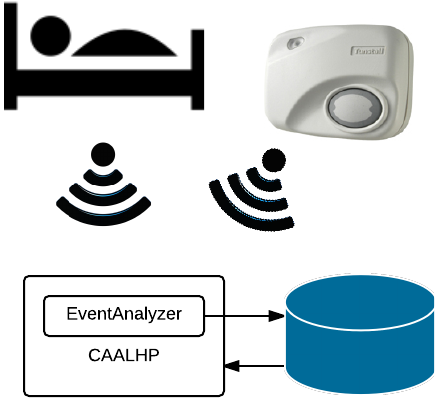
\includegraphics[width = 0.40 \textwidth]{Deployment}
	\caption{Deployment diagram of the system. 
		Each sensor is connected to the CAALHP with a wireless link.
		Inside the CAALHP runs the analyzer module with the False-positive filter in.}
	\label{fig:deployment}
\end{figure}

\begin{figure}[hbtp]
	\centering
	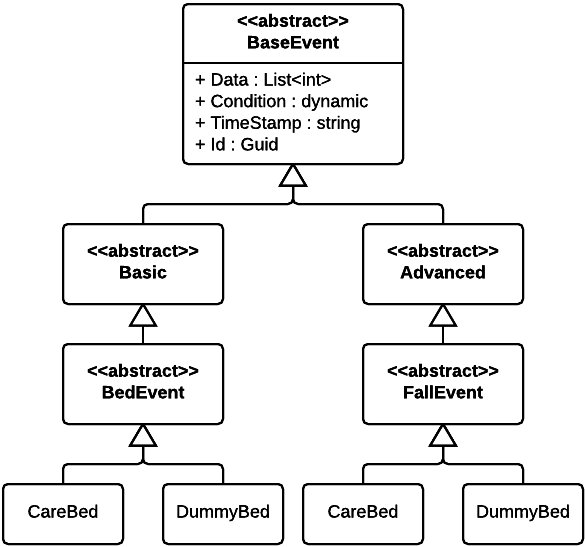
\includegraphics[width = 0.48 \textwidth]{UML}
	\caption{UML diagram of the event classes}
	\label{fig:UML}
\end{figure}


\vspace{-10pt}
\subsection{Evaluation}
\vspace{-15pt}

The program consist of 27 tests, all green, varying from unit testing inserting new elements in the databases, to integration testing calculations of new, incomming events and whether they are stored with correct values.

Besides that is several tests of activating the Shimmer unit tested, while sitting and not sitting in the Carebed, which all gives expected results of the likelyhood of the Shimmer being false-positive or not.



% Building a functional application requires a stable architecture.
% Building a scalable application requires a good architecture, which most of this project is capable of delivering.

% To analyze events, the events must comply as the same types of events\cite{BB-types}.
% Events all inherits from the same class, \texttt{BaseEvent}, which contains properties for data and probability of the event of occurrence.
% If the probability is not debatable (did or did not happen) an inherited class, \texttt{Basic}, converts the probability to a \texttt{bool} from a \texttt{dynamic}, or to probability in the \texttt{Advanced} class as an \texttt{int}.
% Because multiple manufacturers might produces sensors to do the exact same, e.g. register if you are in your bed, a general event for being in you bed is created. \texttt{BedEvent}, inheriting from \texttt{Basic}, allowing specific implementations to be made.
% Here a \texttt{DummyBed} and a \texttt{CareBed} (named by the product) is created inheriting from \texttt{BedEvent}.

% A fall detector bases its event on raw data.
% But since the data does not say either 'fall'/'not fall', it can give a probability of a fall.
% Letting a category of \texttt{FallEvent} inherit from \texttt{Advanced}, a \texttt{DummyFall} and a \texttt{ShimmerEvent} can send raw data as well as a probability to the CAALHP.

% When creating a service to analyze the events, each type of event it should be looking at must be registered.
% This will be done as soon as the class, \texttt{EventAnalyzer}, is initializing by creating new objects of each concrete class, which also will register them as possible entries for the MongoDB.


%!TEX root = Main.tex
\vspace{-5pt}
\section{Discussion}
\vspace{-5pt}

The filter works as first intended.
Events are handled real-time, in a separate process, and it is scalable.
Adding new concrete events and types of events is easy, storing them uses the exact same call the current does, and retrieving likewise.
The architecture of the service is implemented as intended with the requirements.
The actual implementation of probability calculations can be changed to another and better model.

The current model list all events that affects the incoming event, and each of them are searched for in a database for previously occurrence, and only in the timespan.
Each found event will then affect the probability of the new event actually happening.
The formula to calculate the probability is shown here:
\begin{align*}
prob &= oldProb \cdot \dfrac{100 - (condition \cdot plausibilityFactor)}{100} \\
prob &= 90 \cdot \dfrac{100 - (50 \cdot 0.5)}{100} = 67.5\%
\end{align*}
First, the \texttt{condition} is how much the developers meant for the new event to be affected by the existing event.
Second, the \texttt{plausibleFactor} is a static value (in this case 0.5) that prevents events from zeroing a probability.
Third, this value is converted to a percentage of affection, in this example 0.75 and multiplied onto the \texttt{oldProbability}.
\\
This is done for each event that effects the event.

This is not the best method of calculating the new probability of events.
A better option would be a Bayesian Network\cite{MicrosoftBayesian}, which at the first glance the current model could look a bit like it, but far from is.
With a Bayesian Network the model will be able avoid overfitting, improve affection values, and combine prior data for better calculations.
A third options is using a Kalman Filter\cite{welch2006introduction}, to look at previous events, and recursively calculates a new probability.
When more sensors and more affections get added the weight of previous events should scale better than the current model.

The filter can also be improved further by making the super class of the events more generic.
The current implementation uses a list of \texttt{int} and a \texttt{dynamic} for probability.
However, a smarter approach would be making the list either a \texttt{double} or just a \texttt{float} to allow decimal numbers for the data set.
This would allow the Shimmer unit to send its raw data to be calculated in multiple ways and heighten the affection from a static value to a more dynamic calculation.
It would also allow the CareBed to send the actual weight of the person in the bed to the system, which other services and monitors could subscribe and use.

% Adding new event to the filter is equally easy, since the filter will both register the event to look for with the CAALHP and register it in MongoDB in the same call.
% Specifying how the filter should affect the new event, or others should be affected is a single line, and can be added with the concrete type but also the general type for the event.

% I diskussionen er det mere relevant at forholde sig til hvilke andre ting der kan gøres for at forbedre kvaliteten af dit filter. Bayesian networks, ANN, Kalmar, m.v. 

% But simply because the filter works as intended does not mean that the final outcome is perfect, nor that the process to get there was done in the smartest way.
% The major component, that took time was getting MongoDB to work, and understand why it only worked half the time.
% After MongoDB switched from synchronous calls to asynchronous calls, a lot of methods changed names, which meant finding help was more than the regular challenge -- now, close to nobody, had asked the question for a problem with the new API, and the new documentation was still being written and rewritten.
% This meant that those examples MongoDB's website offered could change, both location and structure of dissemination.
% Most of the examples MongoDB's website offered was also written for people who knew what they were doing. 
% This meant that more than halfway through the project I realized I didn't have to convert my objects to \texttt{Bson}, store it, read it, convert it back to my own object's type, but could simply insert my own object, and pull it right back out.

% Another area that coursed trouble was the TTD aspect for MongoDB. 
% When I ran all test by them self they all flagged green.
% But when they were all run together only the first would succeed. 
% Good clues were provided to what was actually wrong, but others with similar problems all had a "oh, I solved it" response and/or never said anything useful regarding their solution.
% Having another person who had tried MongoDB would greatly have improved the time it took to finish this project.

% Other frameworks were considered instead of MongoDB -- \texttt{db4o}\cite{db4o} was considered switching to, since its calls where simple and the project needed simple operations.
% \texttt{NDatabase} was another option quickly considered, but ultimately ditched due to sunk-cost fallacy.
% Both of these frameworks might, in hindsight, have been a better choice given the circumstances.
% The filter performs no hard sorting, needs no caching, or containing lots of subdocuments with more subdocuments in.

% Another area worth looking at will be the algorithm to handle the new probability of occurring events.
% The current algorithm is static and will apply half the weight intended, because multiple events could potential affect the new event.
% But the math could be changed to fit the actual weight, and letting a more generic version of decision.
% Instead of applying the weight based on what happened within a certain time frame, it might be better to apply a function that tells how important previous event are based on the time since they occurred.

% A third thing, which the overall filter lacks, is what happens if the order of the events come into the wrong order.
% If a fall is detected first and no bed event has been detected, it will trigger an alarm.
% But if the bed event comes in after 2 seconds, the alarm will not be stopped.
% A solution to this could be to wait for  \textit{x} seconds before making actual decisions -- but how long should it wait? 
% 2 / 5 / 10 seconds?
% This could be solved by stating the update period for each sensor, e.g. the bed sensor triggers each 2000 millisecond, and therefore all events depending on this must wait this time before making their decision.


% Artikel:
% - Lagdeling
% - Måden at sende beskeder (Carestore's beskedmekanisme -> afkobloing)
% - Context, heirarki, gemt i service
% - Hvordan deles op, hvem beslutter


% \newpage	
% \appendix

% \bibliographystyle{ieeetr}
% \vspace{-5pt}
\printbibliography


\end{document}